\documentclass[aspectratio=169,14pt,t]{beamer}
\usepackage[utf8]{inputenc}
\usepackage[T1]{fontenc}
\usepackage{amsmath,booktabs,graphicx,xcolor}
\graphicspath{{figures/}}

\definecolor{primary}{HTML}{2D5F8B}
\definecolor{deep}{HTML}{1F4566}
\definecolor{gold}{HTML}{C9A24A}

\usetheme{default}
\setbeamercolor{title}{fg=deep}
\setbeamercolor{frametitle}{fg=primary}
\setbeamercolor{structure}{fg=primary}
\setbeamercolor{itemize item}{fg=primary}
\setbeamercolor{normal text}{fg=black}
\setbeamerfont{title}{size=\huge,series=\bfseries}
\setbeamerfont{subtitle}{size=\normalsize}
\setbeamerfont{author}{size=\large}
\setbeamerfont{institute}{size=\normalsize}
\setbeamerfont{date}{size=\normalsize}
\setbeamerfont{frametitle}{size=\Large,series=\bfseries}
\setbeamersize{text margin left=9mm,text margin right=9mm}
\setbeamertemplate{navigation symbols}{}
\setbeamertemplate{itemize item}{\raisebox{0.2ex}{\scriptsize$\blacksquare$}}
\setbeamertemplate{blocks}[default]
\setbeamertemplate{frametitle}{%
  \vskip2.2ex\usebeamerfont{frametitle}\usebeamercolor[fg]{frametitle}\insertframetitle\par
  \vskip0.7ex{\color{gold}\hrule height 1.4pt}\vskip1.6ex}
\setbeamertemplate{footline}{%
  \hspace{9mm}{\footnotesize\color{gray}Dyju \textperiodcentered{} How Much Personal History Is Enough?}%
  \hfill{\footnotesize\color{gray}\insertframenumber/\inserttotalframenumber}\hspace{9mm}\vspace{2.5mm}}
\setlength{\leftmargini}{1.3em}
\addtolength{\itemsep}{0.6em}

\title{How Much Personal History Is Enough?}
\subtitle{Measuring the data requirement for individualised financial behavioural anomaly detection}
\author{Briyan George Dyju}
\institute{Independent Researcher, Dubai, United Arab Emirates}
\date{Independent research, 2026}

\begin{document}

\begin{frame}[plain]
\titlepage
\note{Thank you for having me. I'm Briyan Dyju, an independent researcher in Dubai, and I want to ask a simple question: how much of a person's own history does an anomaly detector need? [0:15] Transition: Let me start with a customer on their first day.}
\end{frame}

\begin{frame}{A new customer opens an account}
\large \begin{itemize}
  \item Personal detector: compare with your own past
  \item Day one: your past is empty
  \item 900 units: normal for one, wild for another
  \item One population rule serves people badly
\end{itemize}
\note{A personalised detector compares each payment with your own past behaviour. That's powerful, because a 900-unit purchase can be ordinary for one person and extraordinary for another. But on day one, there is no past to compare with. [1:15] Transition: So when does the personal baseline start to work?}
\end{frame}

\begin{frame}{Where does the baseline start to work?}
\large \begin{itemize}
  \item Deployed systems filter ``unseasoned users''
  \item The cutoff is assumed, not measured
  \item We found no published measurement
\end{itemize}
\vspace{0.9em}
\begin{center}{\LARGE\bfseries\color{primary} How many transactions are enough?}\end{center}
\note{Production systems handle this with a cutoff. One patent family literally filters out 'unseasoned users'. But we could not find any published measurement of where that cutoff should be, so that is what I measured. [0:45] Transition: Here is how I measured it.}
\end{frame}

\begin{frame}{Measure it with one fixed test window}
\large \begin{itemize}[<+->]
  \item Fixed window: the last 60 transactions
  \item Train on the n just before it
  \item n from 1 to 250, always paired
  \item Anomaly: a stranger's real transaction swapped in
  \item No detector's score defines the labels
\end{itemize}
\note{For every account I hold the last sixty transactions fixed as a test window, and train on the n transactions just before it. To label anomalies without circularity, I swap in a real transaction from a different account, so provenance defines the label, not any detector. [1:15] Transition: Here is what I ran this on.}
\end{frame}

\begin{frame}{Three data layers, six detectors}
\large \begin{itemize}
  \item Berka: 300 real bank accounts
  \item Simulation: 240 people, variability set
  \item TabFormer: 300 entities, synthetic
  \item Mahalanobis, k-NN, forest, autoencoder, z-scores
\end{itemize}
\note{Three layers: real bank accounts from the Berka dataset, a controlled simulation where I set how variable people are, and a second, synthetic card dataset. Six standard unsupervised detectors run on each layer. [0:45] Transition: Now the headline result.}
\end{frame}

\begin{frame}{25 transactions reach 90\% of best}
\begin{columns}[T]
\column{0.65\textwidth}
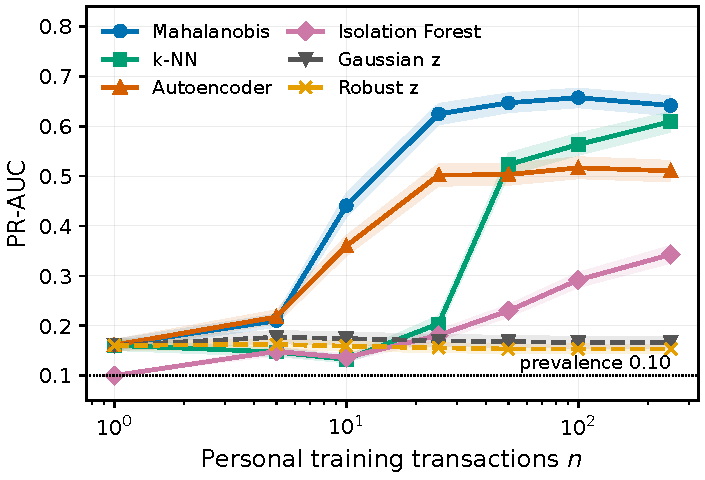
\includegraphics[width=\linewidth,height=0.56\textheight,keepaspectratio]{fig_berka_curves.pdf}
\column{0.33\textwidth}
\vspace{1.2em}
\small \begin{itemize}
  \item Mahalanobis PR-AUC \textbf{0.657}
  \item 98\% of the gain by n = 50
  \item Both z-scores never learn
\end{itemize}
\end{columns}
\note{This is the data-efficiency curve on real bank accounts. The shrinkage Mahalanobis detector reaches ninety percent of its best precision-recall AUC, 0.657, at just twenty-five personal transactions, and has gained almost everything by fifty. The two simple z-scores never learn at all. [1:30] Transition: But that single number depends on how you define sufficiency.}
\end{frame}

\begin{frame}{The threshold depends on the definition}
\begin{columns}[T]
\column{0.50\textwidth}
\vspace{0.6em}
\centering
\renewcommand{\arraystretch}{1.25}\small
\begin{tabular}{lcc}
\toprule
\textbf{Detector} & \textbf{Rel-90} & \textbf{Rel-95} \\
\midrule
Mahalanobis & 25 & 25 \\
Autoencoder & 25 & 25 \\
k-NN & 100 & 250 \\
Isolation forest & 250 & 250 \\
\bottomrule
\end{tabular}
\column{0.46\textwidth}
\vspace{0.6em}
\begin{itemize}
  \item Same 25 at all \textbf{5} cohort seeds
  \item Stability: never met by a learner
\end{itemize}
\end{columns}
\note{Rel-90 is the smallest n that reaches ninety percent of the best value; Rel-95 uses ninety-five. For Mahalanobis it is twenty-five either way, and it is identical across five independent cohort draws. But the stability criterion, spread across people, is never met by any detector that actually learns. [0:45] Transition: Now a question that matters in practice: should you personalise at all when history is thin?}
\end{frame}

\begin{frame}{Below n = 10, trust the crowd}
\begin{columns}[T]
\column{0.65\textwidth}
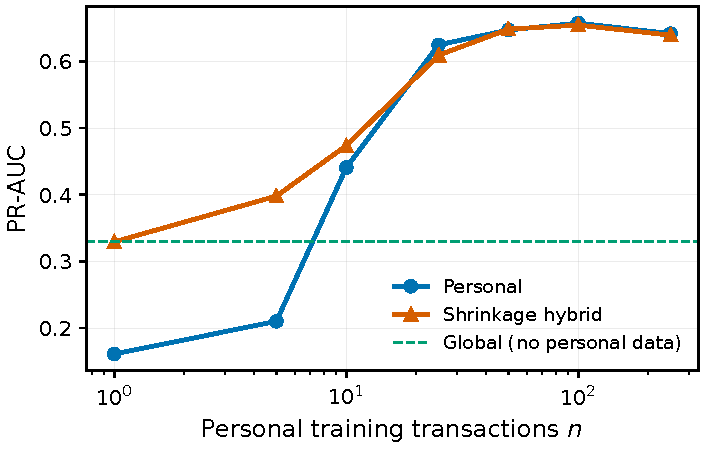
\includegraphics[width=\linewidth,height=0.56\textheight,keepaspectratio]{fig_arms.pdf}
\column{0.33\textwidth}
\vspace{1.2em}
\small \begin{itemize}
  \item Population model: 400 other accounts
  \item Personal worse until n = 10
  \item k-NN: worse until n = 50
\end{itemize}
\end{columns}
\note{The green line is a model built only from four hundred other accounts. Below about ten transactions, that crowd model beats the person's own history. So personalisation is not a safe default in the sparse regime. [1:30] Transition: The orange line shows a fix.}
\end{frame}

\begin{frame}{Shrink toward the crowd}
\begin{center}
{\huge $\mu_h=\frac{n\,\mu_p+\kappa\,\mu_g}{n+\kappa}$}
\end{center}
\vspace{0.4em}
\large \begin{itemize}[<+->]
  \item $\kappa$ = 25, fixed in advance
  \item n = 0: exactly the global model
  \item Never meaningfully worse than either parent
  \item Fails if signal lives in the features
\end{itemize}
\note{The hybrid shrinks the personal estimate toward the population estimate with a weight set only by n. At zero history it is exactly the crowd model, and as n grows it converges to the personal one. In my simulation it fails when the personal signal lives in the features themselves, so it is not a universal cure. [0:45] Transition: Now the part that surprised me most: the alert threshold.}
\end{frame}

\begin{frame}{How you set the alert threshold matters}
\begin{center}
\renewcommand{\arraystretch}{1.05}\footnotesize
\begin{tabular}{lccc}
\toprule
\textbf{n} & \textbf{In-sample flag rate} & \textbf{LOO flag rate} & \textbf{LOO FPR} \\
\midrule
5 & 0.989 & 0.152 & 0.151 \\
10 & 0.960 & 0.012 & 0.007 \\
25 & 0.391 & 0.110 & 0.066 \\
50 & 0.251 & 0.126 & 0.073 \\
\bottomrule
\end{tabular}
\end{center}
\vspace{-0.2em}
\small \begin{itemize}[<+->]
  \item n = 10: \textbf{96\%} flagged in-sample
  \item Leave-one-out: \textbf{1.2\%} flagged
  \item FPR 0.066 at n = 25 (nominal 0.05)
\end{itemize}
\note{A detector needs an alert threshold. If you set it from the model's own training scores, at ten transactions it flags ninety-six percent of everything. With leave-one-out calibration, the same model flags one point two percent. That is an artefact of in-sample scoring, not of data scarcity. [1:30] Transition: Does any of this hold on a different dataset?}
\end{frame}

\begin{frame}{A second dataset reverses a ranking}
\begin{columns}[T]
\column{0.65\textwidth}
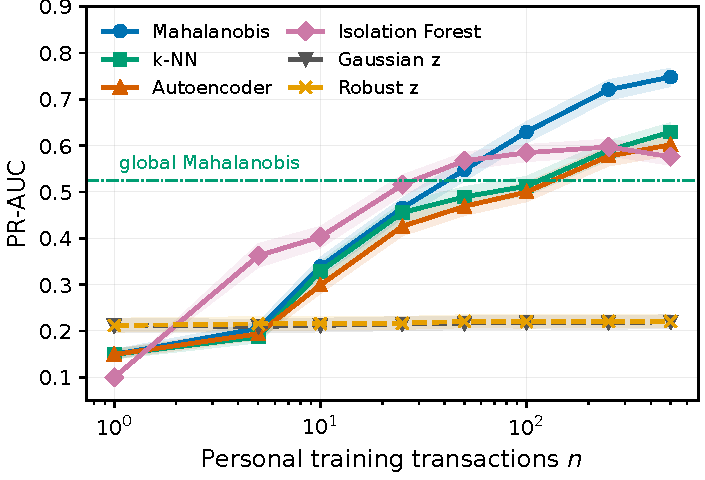
\includegraphics[width=\linewidth,height=0.56\textheight,keepaspectratio]{fig_tabformer_curves.pdf}
\column{0.33\textwidth}
\vspace{1.2em}
\small \begin{itemize}
  \item Same shape, later threshold (250)
  \item Isolation forest best at small n
  \item Worst detector on Berka
\end{itemize}
\end{columns}
\note{On the synthetic card dataset the curve has the same shape, but the threshold moves to two hundred and fifty. And isolation forest, the worst detector on Berka, is the best one at small n here. So which model wins under scarcity depends on the dataset. [1:15] Transition: What makes some people need more history than others?}
\end{frame}

\begin{frame}{Variability sets how fast it learns}
\begin{columns}[T]
\column{0.65\textwidth}
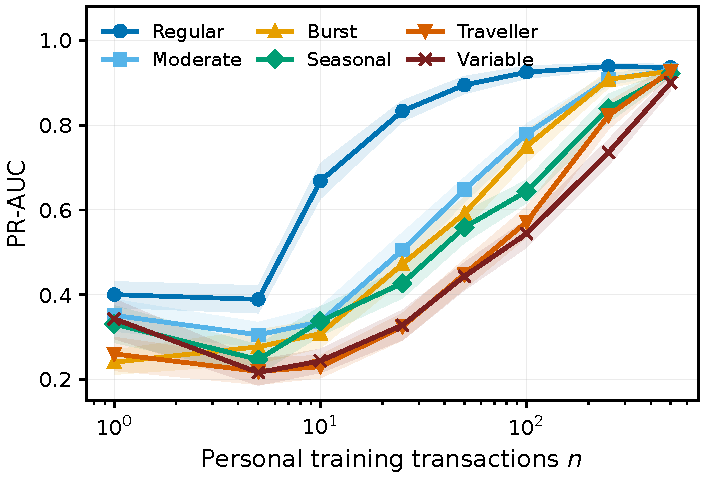
\includegraphics[width=\linewidth,height=0.56\textheight,keepaspectratio]{fig_sim_archetypes.pdf}
\column{0.33\textwidth}
\vspace{1.2em}
\small \begin{itemize}
  \item Regular: 50 transactions; variable: 500
  \item Simulation: Spearman $\rho$ = 0.48 to 0.71
  \item Real accounts: no descriptor predicts it
\end{itemize}
\end{columns}
\note{In the simulation, where I control variability, regular people need about fifty transactions and highly variable people about five hundred. But in the real Berka accounts, none of the eight descriptors I tested predicts an account's requirement. The simulation shows the effect can exist, not that it does in real data. [1:00] Transition: One more practical finding about which history to keep.}
\end{frame}

\begin{frame}{Recent history beats more history}
\large \begin{itemize}
  \item 50 to 250 transactions: 0.647 $\rightarrow$ 0.642
  \item Same 50 from 4$\times$ span: $-$0.036
  \item Drift is real, but doesn't predict loss
  \item $\rho$ = $-$0.08, Holm p = 0.32
\end{itemize}
\note{Going from fifty to two hundred and fifty transactions changes almost nothing, while drawing the same fifty from a four-times-longer span costs a little. I tested the obvious drift explanation directly, and it does not explain which accounts lose. [0:45] Transition: Before I wrap up, what this study cannot tell you.}
\end{frame}

\begin{frame}{Limits and ethics}
\large \begin{itemize}
  \item One bank, 1993 to 1998; second dataset synthetic
  \item 10\% injection far above fraud prevalence
  \item A flag is a deviation, not fraud
  \item Audit is district-level only
\end{itemize}
\note{This is one bank in the nineties, plus a synthetic dataset, and my injected anomalies are far more common than real fraud. A flagged transaction is a deviation, not evidence of fraud. My fairness audit found no district-level gap, but it cannot test age, tenure or immigration status. [0:45] Transition: So what should you take away?}
\end{frame}

\begin{frame}{Takeaways}
\large \begin{itemize}
  \item Baseline ranks well from about 25 transactions
  \item Hybrid removes the cold-start penalty
  \item Calibration moves the operating point
  \item Keep recent history, not all history
\end{itemize}
\note{To summarise: a personal baseline ranks well from about twenty-five transactions; a shrinkage hybrid removes the cold-start penalty; how you calibrate the alert threshold changes the operating point; and recent history is enough. [0:45] Transition: I'm happy to take questions.}
\end{frame}

\begin{frame}{Questions?}
\begin{columns}[c]
\column{0.45\textwidth}
\centering

\includegraphics[height=0.55\textheight]{qr_paper.png}
\column{0.5\textwidth}
{\Large\bfseries\color{primary} Paper and code}\\[0.8em]
\texttt{briyan.xyz/research}\\[0.4em]
\texttt{briyandyju@gmail.com}
\end{columns}
\note{Thank you. The paper is linked at the QR code and I'm happy to take questions. [0:15]}
\end{frame}

\end{document}
